\subsection{Sensors}
The race car being used for this project deploys a high number of sensors, ranging from simple voltage meters on every other battery cell through ride height sensors and all the way to complex pieces of technology like the two \glspl{LiDAR}. For perception of the surroundings and estimating local changes in the state of the car, the most relevant sensors are camera, \glspl{LiDAR}, \gls{IMU}, \gls{INS}, optical sensors and ride height sensors. Some of these need a further explanation, and this is done in the below sections.

\subsubsection{LiDAR}
A \gls{LiDAR} works by sending out a grid of light and timing how long it takes for the light to return. A typical \gls{LiDAR} for autonomous vehicles creates this grid by sending an array of light at a rotating mirror. This means the \gls{LiDAR} covers an entire section of view, both horizontally and vertically. The resolution is set by how many channels it has vertically, how often it sends and receives light and the frequency of rotation. How far it can detect is determined by the sensitivity of the receiver and the power of the sent beam. In a formula student application the allowed power of the emitted light is limited for safety reasons, which means the only real way of extending how far you can detect is by either increasing the sensitivity of your receivers photo detector or by increasing the number of vertical and horizontal channels. The latter will extend the detection range by allowing better outlier rejection, thus reducing the effect of noise at longer distances. 

On board the car are two \glspl{LiDAR}; a Velodyne VL16 with 16 vertical channels and an Ouster OS1 with 64 vertical channels. 

The Velodyne has a vertical resolution of $2.0$\si{\degree} spread across a $360$\si{\degree} \gls{FOV} and a horizontal resolution of $0.1$\si{\degree} around the horizon and going down to $0.4$\si{\degree} towards the limits of it's vertical \gls{FOV}, which is $\pm 15$\si{\degree}. Its range measurements are accurate to $\pm 3$ \si{\cm}, according to the manufacturer. 

The Ouster has a vertical and horizontal resolution of $\pm0.01$\si{\degree}, uniformly spaced around both it's horizontal \gls{FOV} of $36$ degrees and it's vertical \gls{FOV} of $\pm 16.6$\si{\degree}. It has a stated range resolution of $\pm 1.2$ \si{\cm}. Both the \glspl{LiDAR} rotate at 20 \si{\hertz}. 

The OS1 is mounted in the hoop above the driver and scans $360$\si{\degree}, while the VL16 is mounted in front of the front wheels, just under the snout of the car. The idea is that running them in parallel will increase the number of cones detected. 

The placement of the \glspl{LiDAR} can be seen in figure \ref{Fig:SensorPlacementsV2}.


\begin{figure}
    \centering
    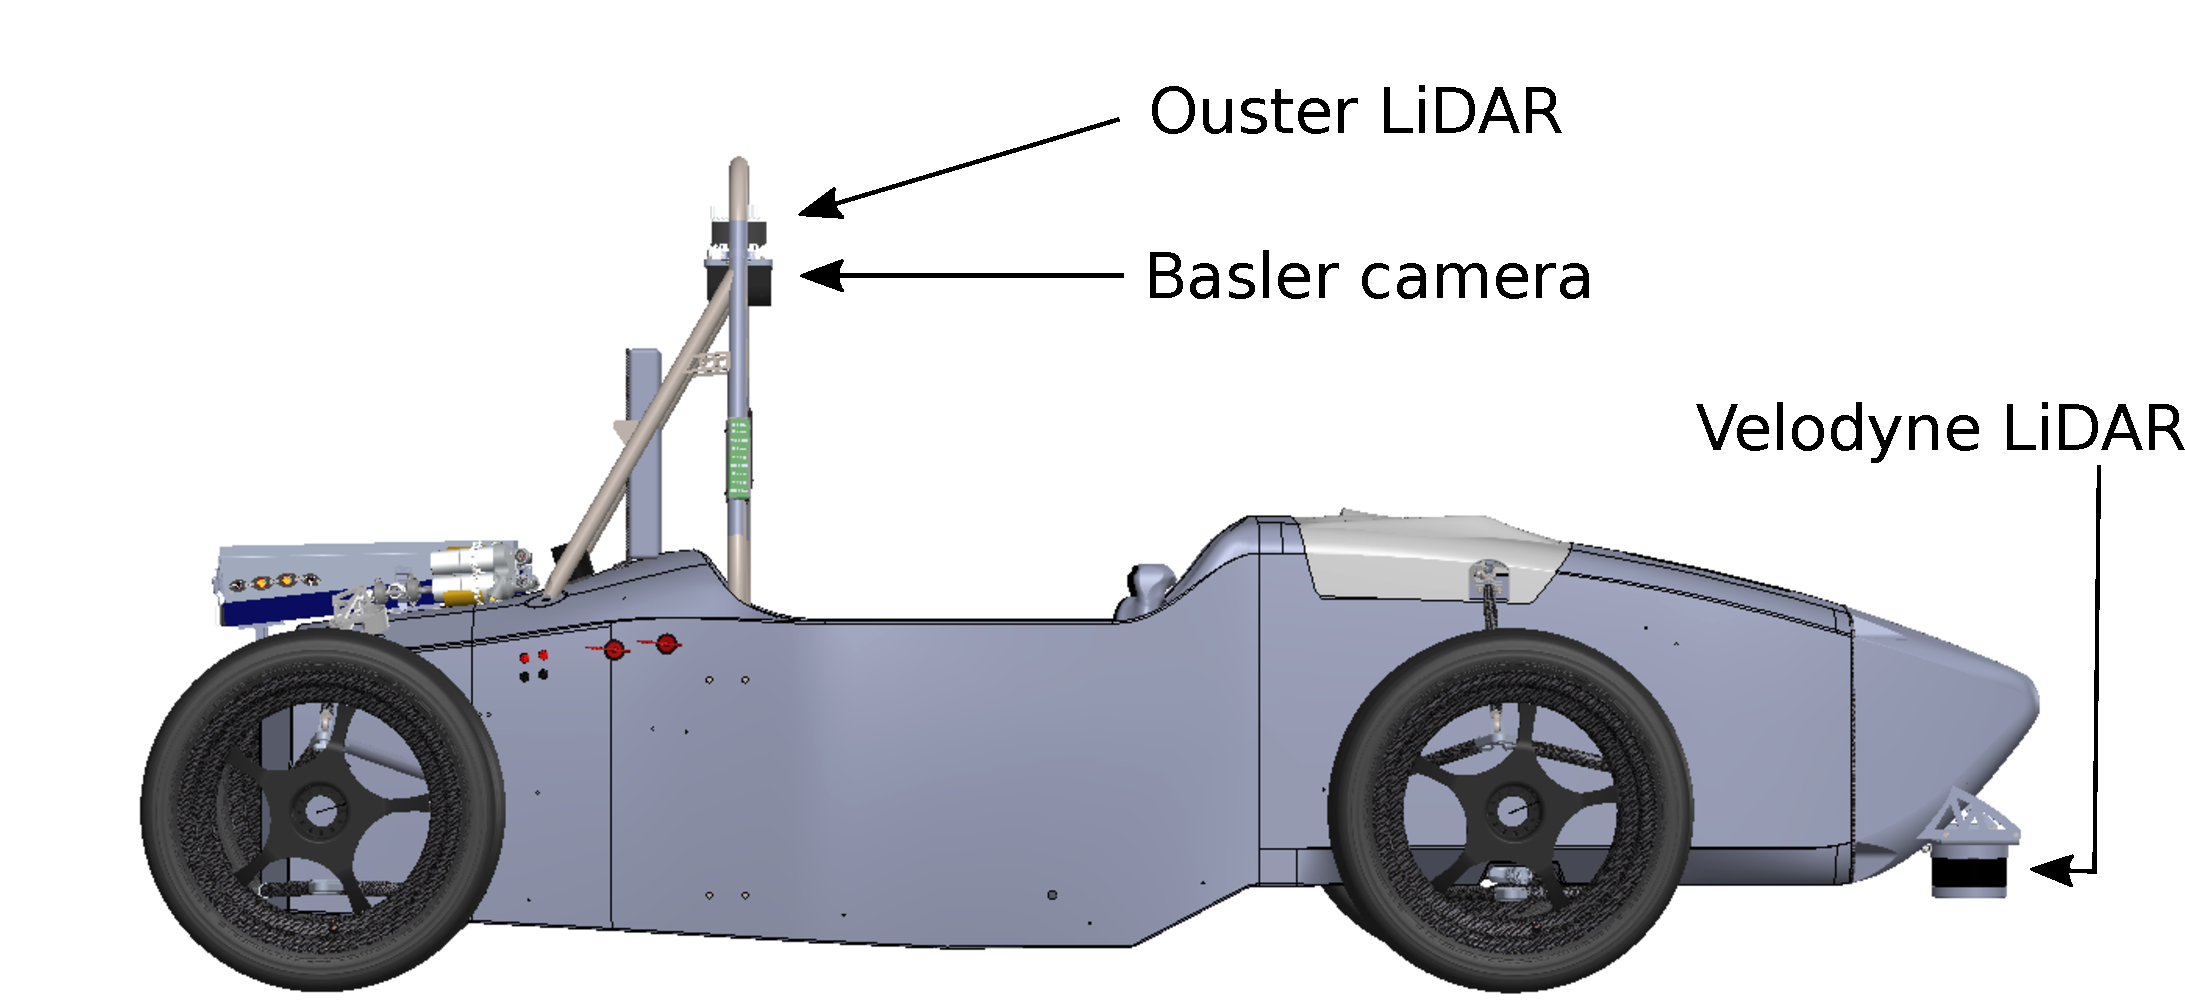
\includegraphics[width=0.8\linewidth]{0_Images/3_Background/SensorPlacements.pdf}
    \caption[Placement of the perception sensors.]{Placement of the perception sensors. A LiDAR and the camera are in the main hoop, while the other LiDAR is below the snout.}
    \label{Fig:SensorPlacementsV2}
\end{figure}

\subsubsection{IMU}
An \gls{IMU} measures acceleration and rate of change in rotation. It typically does so in all three dimensions, amounting to a total of 6 \gls{DOF}. Unless you are buying extremely expensive \glspl{IMU}, it is typically going to be a \gls{MEMS} type \gls{IMU}. 

\gls{MEMS} \glspl{IMU} measure acceleration by having a microscopic mass attached to something elastic, so it is allowed to move in one dimension. When it is influenced by an acceleration parallel to its axis of movement, it will move in that direction. How far it moves is determined by the elasticity of the material, thus giving an indirect measure of how large the magnitude of the acceleration is. The \gls{IMU} measures how much the mass has moved by an elastic material, which has a capacitance that is dependent on the materials deflection. This is then converted to a measure of the acceleration along this dimension, since an empirical relation between capacitance and acceleration has been found through testing. The same is then done for the two other dimensions. 

The rate of change in orientation is measured by the Coriolis effect. The Coriolis effect refers to the fact that a mass with a velocity in a rotating frame of reference will get an acceleration perpendicular to the velocity. A mass in the \gls{IMU} is made to vibrate back and forth, and when the \gls{IMU} has a rate of rotation  with an axis perpendicular to the masses back and forth movement, it will get an acceleration perpendicular to the vibration axis. This acceleration is then measured the same way as for the linear acceleration explained above, and converted to an estimate of the rate of rotation. Since the way the \gls{IMU} measures acceleration of the mass is restricted to one dimension, measuring the three possible dimensions of rotation demand three of these vibrating masses. 

Atmos sports a Vectornav VN300 which is both an \gls{IMU} as well as a \gls{GPS}-receiver. It has a dual antenna setup where the two antennas are aligned with the x-axis of the car. This is done so it can get yaw angle, which the GPS gives out with 2 degrees of error, according to the manufacturer. It has an output rate of 400 \si{\hertz}, and filters internally using a Kalman filter. 

The INS outputs linear accelerations in three dimensions, the rate of change of the yaw, pitch and roll, as well as heading and a quite noisy position data from the GPS. 

Even though these sensors typically are very expensive, they do contain a lot of noise. The \gls{IMU} on the race car therefore uses a Kalman filter, fusing the \gls{IMU} data and information from the two \gls{GNSS} antennas to filter away as much as possible of the noise. Nonetheless, the output is still not good enough to use as a sole source of odometry, as it drifts too quickly.

\subsubsection{Camera}

A camera works by having an array of photo diodes that a lens focuses light from the world onto. The photo diodes then convert the intensity of the light into a digital number. This matrix of intensities is then possible to visualise on a computer as an image, representing the view from the camera at the moment of capture. It also allows a computer to process this image further. In Formula student, cameras as mostly used to find the delimiters of the race track.

An issue when working with cameras is that in order to estimate where something in the image is, one needs to know the transformation between camera and the real world. This implies finding all the points in the real world that each pixel could come from. To find this transformation is to find the intrinsic parameters of the camera, and is usually done by taking photos of something of known dimensions and calculating how the camera distorts these values. Revolve does this using Kalibr\cite{Kalibr1}\cite{Kalibr2}\cite{Kalibr3}. 

On Atmos, there is a Basler PYTHON 1300 camera placed in the main hoop (figure \ref{Fig:SensorPlacementsV2}). This is used for detection of cones, as well as for determining the color of already detected cones. It has a 74.65\si{\degree} field of view and a resolution of 1280 x 1024, running at 200 Hz. To be usable for computer vision at high velocities it has a global shutter, meaning all the photo diodes capture at the same time. This avoids the rolling shutter effect, where the image is distorted due to the velocity of the camera at the moment of capture.

\subsubsection{Optical encoder}

To measure the angle of the steering wheel and the rate of rotation of the four wheels, optical encoders are used. They work by having a light source shine through holes in a disc mounted on the rotating part, centred on the axis of rotation. On the stationary part there are photo diodes, that send out a positive bit when the light hits them. The holes on the disc are made in a special pattern, such that the pattern of bits sent out by the photo diodes makes it possible to know at what angle the disc is currently in. This pattern typically employs a grey encoding\cite{GrayCode} to ensure that only one bit is changed each step. 

A typical optical encoder, the ones used by Revolve NTNU included, has a stated accuracy of $\pm 10$ arc-seconds, which equates to around 0.0028\si{\degree}. This is of course only under ideal circumstances, and does not take into account effects such as concentricity of the glass disk on its hub, perpendicularity of the hub relative to the plane of the optical disk, thermal effects and so on. This is however much better accuracy than what is needed for our applications, as the error stemming from the optical encoder is believed to be dominated by other errors.

The car has optical encoders in each wheel, giving the rate of rotation of the wheels, given in \gls{RPM}. These are then possible to convert to the forward velocity of the wheels, if the wheel radii and slip ratio is known. 

Another optical encoder measures steering wheel angle, which through a lookup table gives out the angle of the front wheels with the x-axis. 

\subsubsection{Ride height sensors}

There are also ride height sensors, that give the linear travel of the shock absorbers. This could be used to compute the height above the ground, but in the authors opinion they are far from accurate enough to be usable.


\subsection{Perception systems}

In order for Atmos to navigate the race track without hitting any delimiters, it needs to know the location of them. This year this is done by three separate systems run in parallel. Two \gls{LiDAR} systems and one camera system. Here is a small intro to how these systems work. Note that both the \gls{LiDAR} systems work the same way and is therefore only explained once.

A visualisation of the output of the two systems can be seen in figure \ref{Fig:LiDARCamViz}.

\begin{figure}
    \centering
    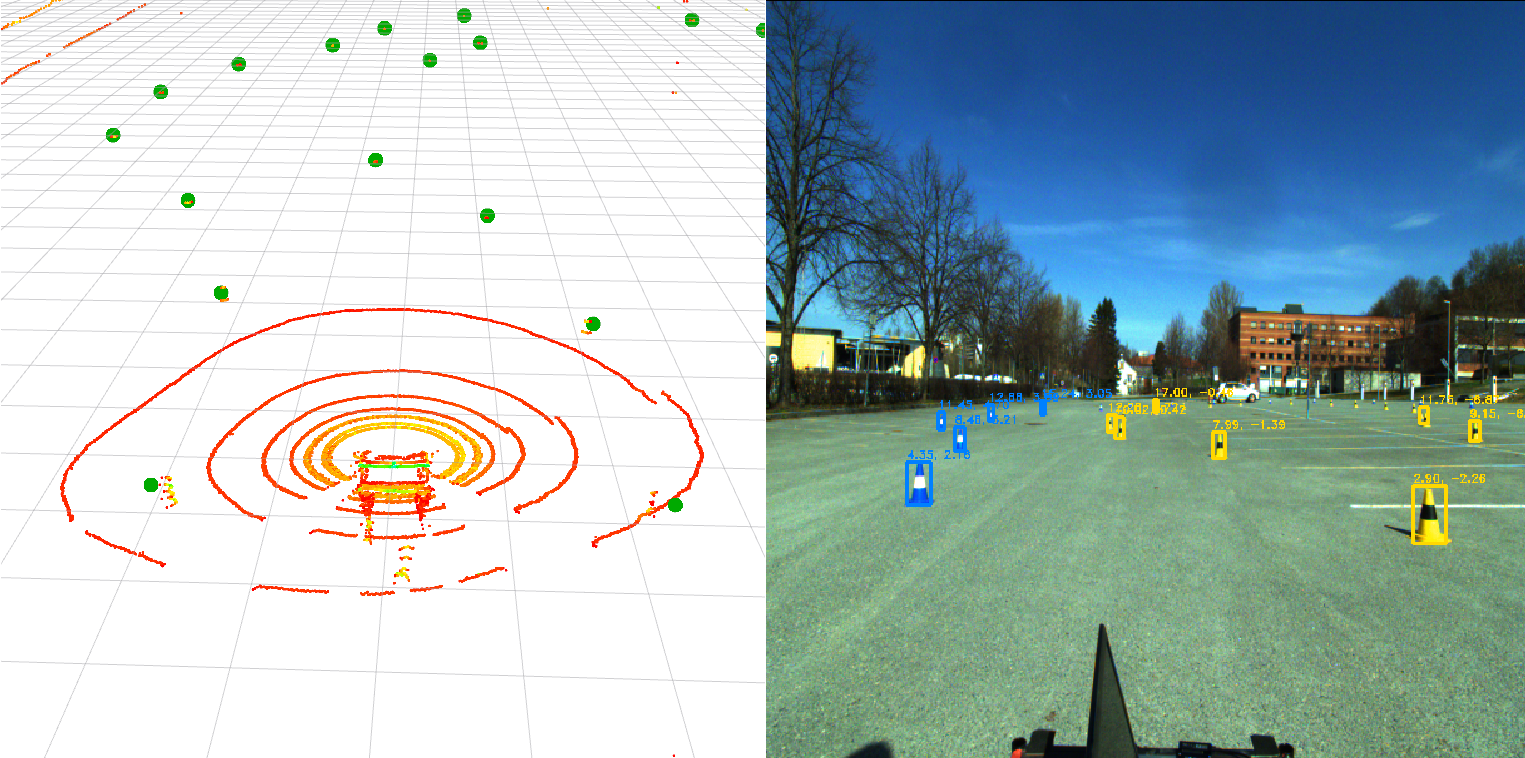
\includegraphics[width=\linewidth]{0_Images/3_Background/LiDARCam.png}
    \caption[Visualisation of the output of the detection systems.]{Visualisation of the output of the detection systems.}
    \label{Fig:LiDARCamViz}
\end{figure}

\subsubsection{LiDAR detection algorithm}
The point cloud coming from the \glspl{LiDAR} get filtered based on position. That means points too low, too high or too far away are discarded. The ground is then removed, following the method used in \cite{GroundRemoval}. The point cloud is then downsampled into a voxel grid and Euclidean clustered, both using functions from the \gls{PCL}\cite{PCL}. The true data in the downsampled clusters are then recreated and the centroid is found. Finally there is an outlier removal, where centroids with neighbours that are too close or too far away are removed. The centroids are then sent to the \gls{SLAM} frontend as a set of detected cones.

The \gls{LiDAR} detection approach is summarised in figure \ref{Fig:LiDARApproach}.

\begin{figure}
    \centering
    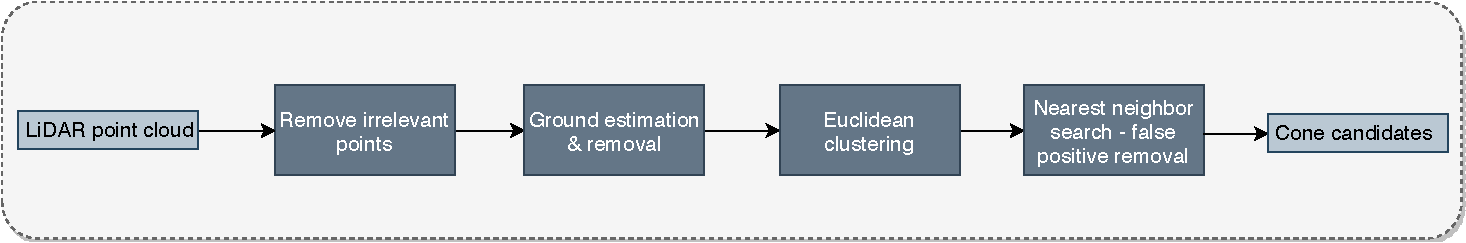
\includegraphics[width=\linewidth]{0_Images/3_Background/LiDARApproach.pdf}
    \caption[Summary of the LiDAR detection algorithm.]{Summary of the LiDAR detection algorithm.}
    \label{Fig:LiDARApproach}
\end{figure}

\subsubsection{Camera detection algorithm}

The images from the camera get fed into a neural net built on \gls{YOLO} V3\cite{YOLOV3}. The last few layers of the net have been retrained on a quite extensive labelled data set of cones, built up over the last two years by trading with other teams. This net outputs bounding boxes on cones in the image, as well as the color of the detected cones. 

The bounding boxes are then used to find the position in the body frame of the detected cones. Two methods have been tested for this. The first is using only geometry \cite{BBGeometry}, considering the size and position of the bounding box. The second solution is to send the bounding boxes and the geometrically estimated positions into another neural net that corrects the initial estimate \cite{PosNeuralNetCorrection}. 
